\documentclass{llncs}
\usepackage{graphicx}
\usepackage{url}
\usepackage{subfig}
\usepackage{tabularx}

% --- TITLE AND AUTHOR INFORMATION
\title{Detecting Bot Behaviour in Social Media \\ using Digital DNA Compression}
\author{Nivranshu Pasricha \and Conor Hayes}
\institute{Insight Centre for Data Analytics \\ Data Science Institute \\ National University of Ireland Galway \\
\email{\tt name.surname@insight-centre.org} }
% --- END OF PREAMBLE 

% --- START DOCUMENT
\begin{document}
\maketitle

\begin{abstract}
A major challenge faced by online social networks such as Facebook and Twitter is the remarkable rise of fake and automated bot accounts over the last few years. Some of these accounts have been reported to engage in undesirable activities such as spamming, political campaigning and spreading falsehood on the platform. We present an approach to detect bot-like behaviour among Twitter accounts by analyzing their past tweeting activity. We build upon an existing technique of analysis of Twitter accounts called Digital DNA. Digital DNA models the behaviour of Twitter accounts by encoding the post history of a user account as a sequence of characters analogous to an actual DNA sequence. In our approach, we employ a lossless compression algorithm on these Digital DNA sequences and use the compression statistics as a measure of predictability in the behaviour of a group of Twitter accounts. We leverage the information conveyed by the compression statistics to visually represent the posting behaviour by a simple two dimensional scatter plot and categorize the user accounts as bots and genuine users by using an off-the-shelf implementation of the logistic regression classification algorithm.

\keywords{Social Media $\cdot$ Twitter $\cdot$ Online Social Networks}

% \keywords{First keyword  \and Second keyword \and Another keyword.}

\end{abstract}

\section{Introduction}

Twitter is a popular online social network with 139 million average daily active users (DAU) \cite{twitter_quarterly_results_2019}. It has become one of the largest sources of news in the world over the last few years. Twitter was launched in 2006 with the idea of using an SMS service to send messages to other people in a group. Registered users can post short messages of up to 280 characters (increased from 140 characters in 2017) called tweets on the platform through different means including the Twitter website, native smartphone \& desktop applications and other third-party client applications.

Twitter's API (Application Programming Interface) allows programmers and developers to create services and applications which can be programmed to read tweets from other users or automatically post tweets to a user's feed. This makes Twitter a breeding ground for a variety of automated software agents, also called bots, which can interact with other users on the platform. These bots are primarily used for harmless activities such as \texttt{@year\_progess}\footnote{\url{https://twitter.com/year_progress}}, a bot account that posts passage of time in an year as a progress bar and \texttt{@MuseumBot}\footnote{\url{https://twitter.com/MuseumBot}}, an account that posts random images from the Metropolitan Museum of Art. Some bot accounts such as \texttt{@EarthquakesSF}\footnote{\url{https://twitter.com/EarthquakesSF}} spread helpful content in the time of disasters like earthquakes and another bot account \texttt{@tinycarebot}\footnote{\url{https://twitter.com/tinycarebot}} posts reminders for self care actions to its followers. However, there have been instances in the recent past where bot accounts have been accused of malpractices such as spamming \cite{lee2011seven}, spreading misinformation \cite{shao2018spread}, amplifying misconceptions \cite{doi:10.2105/AJPH.2018.304567} and manipulating political discussions \cite{FM7090}.

Detecting automated bot accounts or bot-like behaviour on Twitter has become a topic of interest among academics and researchers over the last few years. Since this task includes analyzing thousands of accounts and millions of tweets, it is unfeasible for humans to do this quickly and efficiently. The task of bot detection can be modelled as a supervised learning task where Twitter accounts can be classified into one of two categories of bots and genuine users. A supervised machine learning or a deep learning classification algorithm can be used to train a model on a labelled dataset with appropriate features such as user profile attributes and past tweeting activity in order to identify accounts as genuine users or bots with high accuracy.
\\

The main contributions of this paper are as follows:

\begin{itemize}

\item To classify Twitter accounts as bots or genuine users, we start with the assumption that the long-term behaviour of a bot account on Twitter is less random than the behaviour of a genuine user, or in other words, the behaviour of a bot account is more predictable. We measure this randomness and unpredictability in the posting behaviour of a Twitter account by employing a lossless compression algorithm on the Digital DNA sequence of the account. The technique of Digital DNA was designed in \cite{7876716} to encode the posting history of a Twitter account as a sequence of characters, just like the actual human DNA sequence. 

\item We use this string compression approach on a group of Twitter accounts and obtain compression statistics, namely the size of the uncompressed DNA sequence, the size of the compressed DNA sequence and the value of the compression ratio. These compression statistics are then used as a measure of randomness and predictability in the behaviour of the accounts under study.

\item Based on the compression statistics, we present a 2-dimensional scatterplot as a visual representation of the predictability in the behaviour of a group of Twitter accounts.

\item We then use the compression statistics as features in a supervised machine learning algorithm and learn to classify Twitter accounts as bots and genuine users.

\item Finally, we evaluate the machine learning model using various scoring metrics and compare them with existing state-of-the-art techniques of bot detection.

\end{itemize}

\section{Related Work}

The issue of dealing with bot and automated accounts on Twitter has become a hot topic in recent years. Various studies and experiments have been carried out to automatically identify bot accounts and study their impact on other users of the online platform. All the existing bot detection techniques in the literature look to identify a combination of features related to user profile, tweet/retweet content and past tweeting activity of the user in order to look for patterns that can be used to distinguish bot accounts from genuine users on the platform.

A framework to identify social bots on Twitter was presented in \cite{varol2017online} which deployed more than one thousand features to train a classifier on a dataset containing Twitter bots and human users. The features used for the task of classification were categorized into one of six categories of user meta-data features (number of friends and followers, counts of tweets, retweets and replies, profile description etc.), friends features, network features, temporal features (number of tweets posted in a fixed time interval and distribution of time intervals between posts), sentiment features and content features (statistics about the length and the entropy of the text of the tweet). The sentiment and content features extracted from the tweets were found to be important features along with the statistical properties of retweet networks for the tweets posted by the accounts.

Another approach proposed to identify bot accounts on Twitter divided a dataset of Twitter accounts into 4 distinct bands (1K, 100K, 1M and 10M) depending upon the number of followers of an account \cite{gilani2017classification}. A Random Forest classifier was then trained using a set of 21 features to classify the accounts either as a human or a bot. General features related to an account such as the age of the account, the count of tweets, retweets, replies and favourites, the tweeting frequency, friend-to-follower ratio and source of Twitter activity were used along with a few novel features such as the count of URLs per tweet, the type of device used for tweeting and the size of the media content posted by an account.

Instead of categorizing Twitter accounts into two groups of humans and bots, the authors in \cite{chu2012detecting} proposed a system to classify the accounts to one of three categories - human, bot and cyborg. A cyborg account here referred to either a bot-assisted human or a human-assisted bot. This system consisted of four major components - an entropy component that used tweeting interval as a measure for behavioural complexity of the account, a spam detection component that looked for patterns in the content of the tweets posted by an account, an account properties component to study the account properties like device information, and a decision maker which used a combination of the features generated by the other components to finally assign a label to an account. The authors also created a metric called account reputation, which was defined as the normalized ratio for the number of accounts followed by a Twitter account and the number of accounts befriended by that account. Human accounts were found to have highest values of account reputation, closely followed by cyborg accounts and bot accounts had much lower values, typically less than 0.5. In terms of frequency of posting tweets, bots were found to exhibit burstiness, i.e., posting a number of tweets in a small interval of time interspersed with long periods of hibernation whereas tweets posted by human accounts had large intervals (typically hours or days) between successive tweets. Bot accounts also exhibited regular posting behaviour while human accounts displayed more complex posting behaviour and higher entropy.

Most of these approaches have been trained to classify accounts using a supervised learning algorithm, however some unsupervised approaches have also been studied for this task. A methodology to identify spam campaigns on Twitter and Facebook modelled a set of user profiles using a weighted social graph where users were inter-linked based on values of a predefined set of 14 features \cite{ahmed2013generic}. The social graph was then clustered using Markov clustering into groups of users that exhibit similar behaviour and activities.

It has been argued that a paradigm-shift \cite{Cresci:2017:PSS:3041021.3055135} has taken place over the last few years in the behaviour of Twitter bots where more sophisticated social bots have been identified that have been able to fool traditional bot detection techniques as well as human annotators. These novel social spambots appear to behave as genuine users when looked at individually, however they exhibit patterns of similar activity when considered as part of a group. A methodology titled ``Social Fingerprinting" was proprosed in \cite{7876716} to identify such sophisticated bots not at individual level but rather as groups of accounts that exhibit similar behaviour. The technique which is inspired by bioinformatics encoded the behaviour of an account as a sequence of bases, represented using a predefined set of alphabet of finite cardinality consisting of letters such as \texttt{A}, \texttt{C}, \texttt{G} and \texttt{T}. This sequence is said to be the digital DNA sequence for an account. One such encoding scheme assigns the type of post (tweet, reply or retweet) made on Twitter to a unique character. The tweets, replies and retweets posted by an account are mapped to characters \texttt{A}, \texttt{C} and \texttt{T} respectively to generate the digital DNA string for the account. 

\[ 
\mathbf{B}^{3}_{type} = 
\left \{
  \begin{tabular}{l}
  $\texttt{A} \leftarrow \textrm{tweet}, $ \\
  $\texttt{C} \leftarrow \textrm{reply}, $ \\
  $\texttt{T} \leftarrow \textrm{retweet} $
  \end{tabular}
\right \}
\]

An approach similar to digital DNA was proposed in \cite{Kan2013} to study the temporal evolution of users in online forums. A feature space was defined to visually represent chronological user events (posts and replies in forum threads) as paths and to model the distribution of inter-event times in order to define a clustering of various online forums. 

The authors in \cite{7876716} define the length of the longest common substring (LCS) or the length of the k-common substring in the digital DNA sequences as a measure of similarity for the two categories of bot and genuine user accounts on Twitter. For a group of accounts consisting of genuine users, the length of the LCS of the digital DNA strings was found to be very short. However, for a group of bot accounts, the length of the LCS was much longer. This idea was then used to identify bot accounts in a mixed group of user accounts which contained accounts for both genuine users and bots by finding the k-common substring for all those accounts and then finding a cut-off, the number of accounts which share a long common substring and classifying all such accounts which share that substring as bots and other accounts with shorter common substrings were classified as genuine human users. Based on this idea, two techniques, one supervised and another unsupervised were further discussed to find of groups of similarly-behaved accounts among a mixed set of accounts of automated bots and genuine human users, both of which showed promising results and were found to be better than the existing state-of-the-art techniques for the task of bot detection.


\section{Dataset}

We use the dataset\footnote{\url{http://mib.projects.iit.cnr.it/dataset.html}} created in \cite{Cresci:2017:PSS:3041021.3055135} to analyze our approach for detecting bot accounts on Twitter. This dataset contains a random sample of genuine human user accounts on Twitter along with a variety of bot accounts. The data was collected over a period of a few months in 2014 and contains profile information for 11017 accounts with more than 6 million posts (tweets, retweets and replies) made by those accounts. The bot accounts in this dataset are broadly categorized into three categories, namely, social spambots, traditional spambots and fake followers. Table \ref{tab:datastats} contains the description of the accounts across the various categories. The authors in \cite{7876716} created two test sets, \texttt{Mixed1} and \texttt{Mixed2} from this dataset to study their approach of Digital DNA and Social Fingerprinting for identifying bot accounts on Twitter. \texttt{Mixed1} contains a random sample of genuine user accounts and a subset a social spambot accounts. These bot accounts were found to be created to target Mayoral elections in Rome, Italy. Around 1000 automated accounts were found to be created by a social media marketing firm to promote and publicize the campaign and policies for one of the candidates. \texttt{Mixed2} also contains a random sample of genuine user accounts and a different subset of social spambot accounts. The bot accounts in \texttt{Mixed2} were found to be created primarily for promotion and advertisement of products on the popular E-commerce platform \url{amazon.com}. The bot accounts categorized as social spambots in Table \ref{tab:datastats} exhibited properties which differed vastly from other known traditional bot accounts. These accounts appeared much more sophisticated than traditional bot accounts and appeared to be operated by genuine human users. The profiles of these social spambot accounts displayed detailed information such as profile pictures, bio, location etc., although most of it was found to be either fake or stolen from other accounts. We evaluate our approach of bot detection using DNA compression on both \texttt{Mixed1} and \texttt{Mixed2} test sets.

\begin{table}
\caption{Statistics for bot accounts and genuine user accounts in the dataset.}\label{tab:datastats}
\begin{tabularx}{\textwidth}{X l r}
\hline
\textbf{Dataset} & \textbf{Description} & \textbf{\# Accounts }\\
\hline
Genuine Accounts & Human-operated Accounts & 3474 \\
 \hline
 Social Spambots \#1 & Retweeters of an Italian political candidate & 991\\
 Social Spambots \#2 & Spammers of paid apps for mobile devices. & 3457\\
 Social Spambots \#3 & Spammers of products on amazon.com. & 464\\
 \hline
 Traditional Spambots \#1 & Spammers of phishing and malicious URLs. & 1000\\
 Traditional Spambots \#2 & Spammers of scam URLs. & 100\\
 Traditional Spambots \#3 & Spammers of job offers. & 433\\
 Traditional Spambots \#4 & Spammers of job offers. & 1128 \\
 \hline
 Fake Followers & Accounts to inflate follower numbers & 3351 \\ 
 \hline
\end{tabularx}
\end{table}

\section{Methodology}

In this section, we describe the methodology used to model past activity and behaviour of Twitter users as a DNA sequence. We also explain our assumptions and reasoning behind the idea of using string compression on these DNA sequences. Furthermore, we describe our strategy to visually represent genuine user accounts and bot accounts based on the compression statistics and how we use this information to classify the accounts using a simple classification algorithm like logistic regression.

\subsection{Compression of Digital DNA}
We start with the assumption that the behaviour of a bot account is more predictable and less random than the behaviour of a genuine human-operated account. To measure the predictability in the behaviour, we make use of digital DNA sequences.
The digital DNA sequence for a user account can be created using an alphabet set of cardinality 3 with symbols \texttt{A}, \texttt{C} and \texttt{T} corresponding to a tweet, a retweet and a reply respectively. This provides a way of representing an account's posting history by encoding the information of past posting activity in a compact and concise fashion. The DNA sequence can be generated for an account by starting with an empty string and scanning through the post history of the account in chronological order, appending the relevant alphabet to the string based on the type of post made by the account. For example, a series of 10 consecutive posts made by an account can be represented by the vector, $\vec s = \left< \texttt{A}, \texttt{C}, \texttt{T}, \texttt{C}, \texttt{A}, \texttt{T}, \texttt{T}, \texttt{T}, \texttt{T}, \texttt{A} \right>$ or alternatively, by the string \texttt{s} $=$ ``\texttt{ACTCATTTTA}". 

In Information Theory, the concept of entropy is used as a measure of randomness in a data signal. It is well known that data with high entropy cannot be compressed and decompressed with high efficiency using a lossless compression technique \cite{mackay2003information}. We compress the digital DNA sequences with a lossless compression algorithm and obtain compression statistics such as the size of the compressed string and the compression ratio which serve as metrics to measure the predictability of an account's behaviour.

\begin{table}
\caption{\label{tab:compression_stats} Mean $(\mu)$ and standard deviation $(\sigma)$ for the length $(L)$, size (in bytes) before compression $(S)$, size (in bytes) after compression $(C)$ and compression ratio $(R)$ for accounts in \texttt{Mixed1} and \texttt{Mixed2}.}
\begin{tabularx}{\textwidth}{X c c c c c c c c}
\hline
 & $L_\mu$ & $L_\sigma$ & $S_\mu$ & $S_\sigma$ & $C_\mu$ & $C_\sigma$ & $R_\mu$ & $R_\sigma$ \\
\hline
Bot Accounts & 703.81 &  1031.26 &  736.81 &  1031.26 &  71.55 &  52.19 &  10.53 &  15.28 \\ 
Genuine Users & 2621.76 &  1002.08 &  2654.76 &  1002.08 &  612.63 &  243.62 &  4.43 &  2.00 \\
\hline
All Accounts & 1050.29 &  1263.80 &  1083.29 &  1263.80 &  169.30 &  237.25 &  9.43 &  14.06 \\
\hline
\end{tabularx}
\end{table}

The digital DNA strings are compressed using the \texttt{zlib} compression library in the Python programming language with default parameters. It is essential to convert a string of ASCII characters into a bytes object in memory before calling the \texttt{zlib.compress()} compression function. The \texttt{sys} module in Python offers a built-in function \texttt{getsizeof()} which returns the size in bytes of an object stored in memory. The value of the compression ratio for a string is then computed as the ratio of the size (in bytes) of the uncompressed bytes object and the size (in bytes) of the compressed bytes object in memory. 

Table \ref{tab:compression_stats} shows the mean and standard deviation for the values of the compression statistics for the two groups of bots and genuine users as well as the combined statistics for all accounts in \texttt{Mixed1} and \texttt{Mixed2} datasets. The average value of the compression ratio for the DNA sequences of bot accounts across the two datasets is $10.53$, while for the DNA sequences corresponding to the accounts of genuine users, the mean value of compression ratio is $4.43$. This is in agreement with our assumption that the behaviour of a bot account is more predictable and less random compared to the behaviour of a genuine human user, hence the higher value of compression ratio.

\begin{figure}
\centering
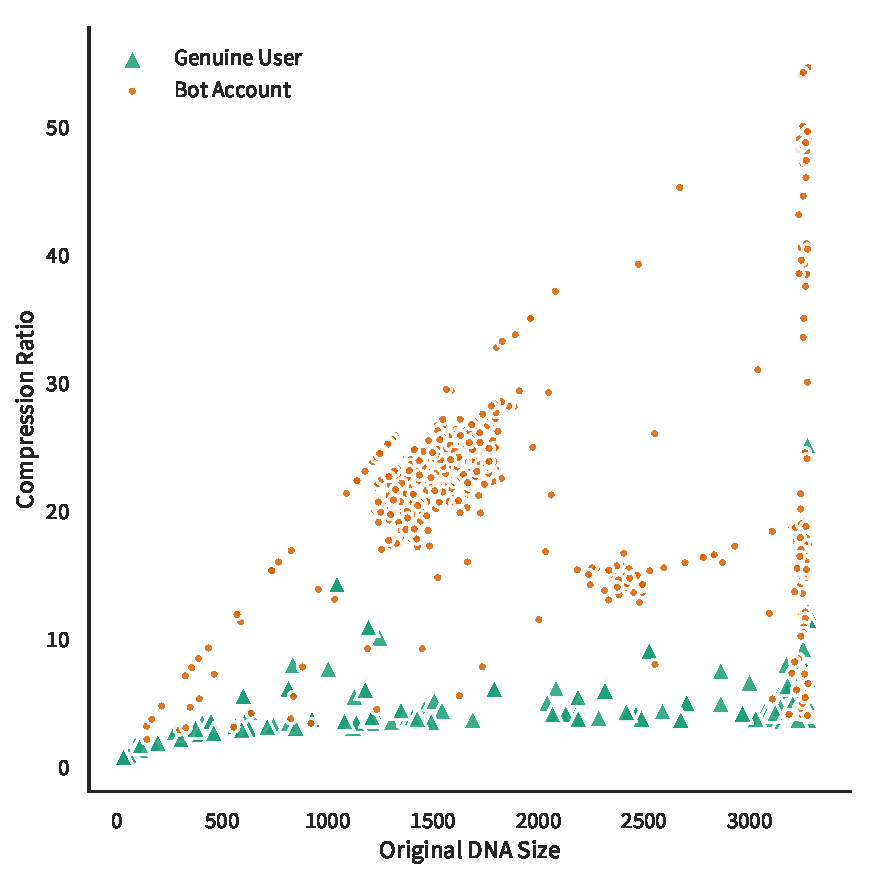
\includegraphics[width=0.6\textwidth]{figures/dna-scatter-2.pdf}
\caption{Compression statistics for Digital DNA sequences corresponding to Twitter accounts in \texttt{Mixed1} and \texttt{Mixed2}. }
\label{fig:compression_stats}
\end{figure}

\subsection{Visualizing Compression Statistics}
Our approach of using string compression on Digital DNA strings presents us with a way to easily visualize the behaviour for a group of accounts using a simple two dimensional scatterplot, as shown in Figure \ref{fig:compression_stats}. Each point in the plot represents an account from \texttt{Mixed1} and \texttt{Mixed2} with the X-coordinate representing the size of the original DNA string in bytes and the Y-coordinate representing the value of the compression ratio.

% \caption{Compression statistics for \texttt{Mixed1} and \texttt{Mixed2}. Each point corresponds to a Twitter account where the X-coordinate represents the size of the uncompressed digital DNA string (in bytes) and the Y-coordinate represents the value of the compression ratio. }

\subsection{Classification with Logistic Regression}
It can be seen in Figure \ref{fig:compression_stats} that a line of separation exists between the bot accounts and genuine human-operated accounts in the dataset under study. The value of compression ratio is typically smaller than 10 for genuine users while bots appear to have much higher value, especially for longer DNA sequences. This implies that a linear classification algorithm can be trained on some labelled data to estimate the line separating the accounts into two classes of bot and genuine user accounts. We split both \texttt{Mixed1} and \texttt{Mixed2} in the ratio of 50:50, where we use $50\%$ of the accounts in the dataset for training and the remaining $50\%$ for evaluation. We use the sklearn \cite{scikit-learn} implementation of logistic regression for binary classification with the default parameters to train two different models, each with two features. We keep the original DNA size as one of the features in both classifiers and use the size of the compressed DNA as the other feature in one of the models and use the compression ratio as the second feature in the other classification model.\footnote{Our code is available at \url{https://github.com/pasricha/bot-dna-compression}.}

\section{Results}

We compare the results obtained with our approach to the results in \cite{7876716} on the same test sets and using the same evaluation metrics - Accuracy, Precision, Recall, F-Measure (F1), Matthews Correlation Coefficient (MCC) and Specificity (True Negative Rate). We randomly pick $50\%$ of the accounts from \texttt{Mixed1} and \texttt{Mixed2}, which we use to train a binary logistic regression classifier with compression statistics as the features and test on the remaining $50\%$ of the accounts in the dataset. We repeat this 1000 times and report the average value for each evaluation metric in Table \ref{tab:eval}.

\begin{table}
\scriptsize
\caption{\label{tab:eval} Comparison of our bot detection technique based on String Compression with the k-Common Substring technique from \cite{7876716}. Results marked in bold are significantly better than both supervised and unsupervised versions of the k-common substring technique $(p < 0.05)$. }
\begin{tabularx}{\textwidth}{{X}*{7}{c}}
\hline
\multicolumn{1}{c}{Technique} &
\multicolumn{6}{c}{Metrics} \\
\hline
 & \tiny{Accuracy} & \tiny{Precision} & \tiny{Recall} & \tiny{F-Measure} & \tiny{MCC} & \tiny{Specificity} \\
 \hline
\textbf{\texttt{Mixed1}} & & & & & & \\
k-Common Substring - Unsupervised \cite{7876716} & 0.976 & 0.982 & 0.972 & 0.977 & 0.952 & 0.981 \\
k-Common Substring - Supervised \cite{7876716} & 0.977 & 0.982 & 0.977 & 0.977 & 0.955 & 0.981 \\
String Compression - Compressed DNA Size & \textbf{0.980} & 0.978 & \textbf{0.981} & \textbf{0.980} & \textbf{0.960} & 0.978 \\
String Compression - Compression Ratio & \textbf{0.984} & \textbf{0.992} & 0.976 & \textbf{0.984} & \textbf{0.968} & \textbf{0.992} \\
\hline
\textbf{\texttt{Mixed2}} & & & & & & \\
k-Common Substring - Unsupervised \cite{7876716} & 0.929 & 1.000 & 0.858 & 0.923 & 0.867 & 1.000 \\
k-Common Substring - Supervised \cite{7876716} & 0.970 & 0.978 & 0.961 & 0.970 & 0.940 & 0.979 \\
String Compression - Compressed DNA Size & 0.967 & 0.982 & 0.950 & 0.966 & 0.935 & 0.983 \\
String Compression - Compression Ratio & \textbf{0.977} & 0.992 & 0.960 & \textbf{0.976} & \textbf{0.954} & 0.992 \\
\hline
\end{tabularx}
\end{table}

Our simple approach to model account behaviour using a compression algorithm on the digital DNA sequence allows us to accurately distinguish between bot accounts and genuine users. For the \texttt{Mixed1} test set, the classifier which uses the compressed DNA size as one of the features, slightly outperforms both the supervised and the unsupervised versions of the k-common substring technique with respect to accuracy, recall, F1 and MCC scores. The other classifier which uses compression ratio and the size of the original uncompressed DNA as the two features, is significantly better than the k-common substring technique for all metrics except recall. In the case of the \texttt{Mixed2} dataset, the classifier with the size of the compressed DNA performs slightly worse than the k-common substring techinque. However, the other classifier is better in terms of 3 of the 6 evaluation metrics, namely, accuracy, F-Measure and MCC. In terms of complexity and scalability, our approach provides a fast and simple way for assessing the predictability in the behaviour of Twitter accounts because compression of a string can be performed in linear time and constant memory overhead.

% Plot for maximum sequence length.
\begin{figure}
    \centering
    \subfloat[\texttt{Mixed1}]{{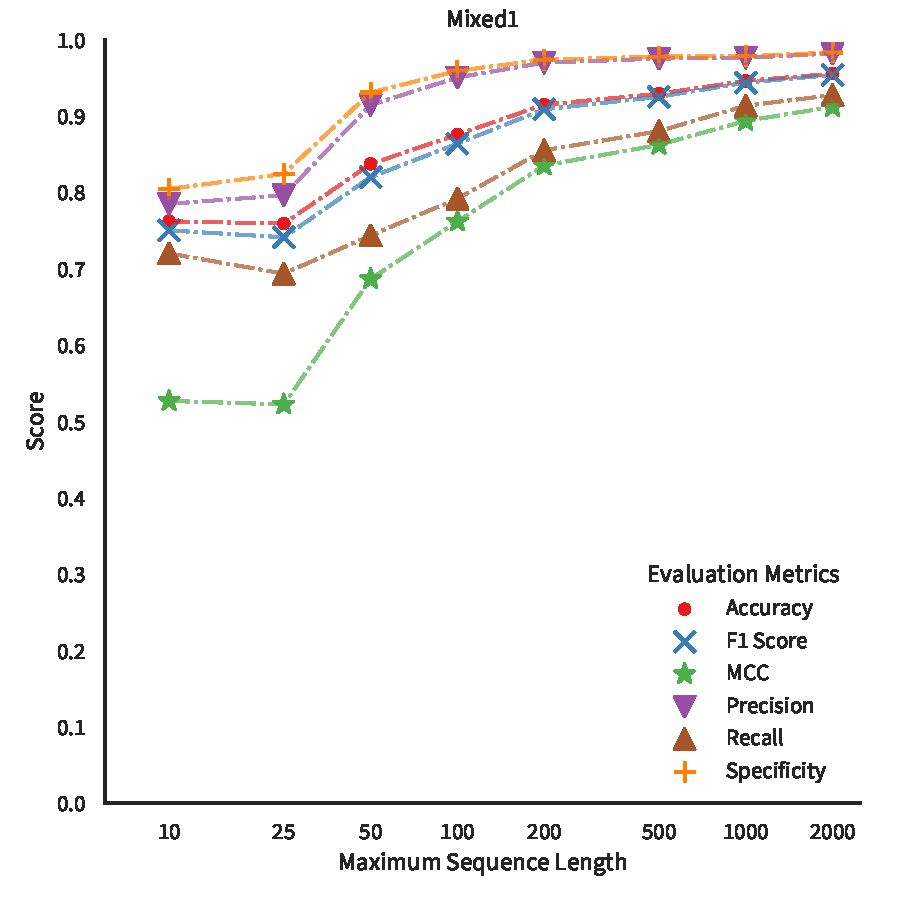
\includegraphics[width=5.5cm]{figures/dna-len-1.pdf} }}
    \qquad
    \subfloat[\texttt{Mixed2}]{{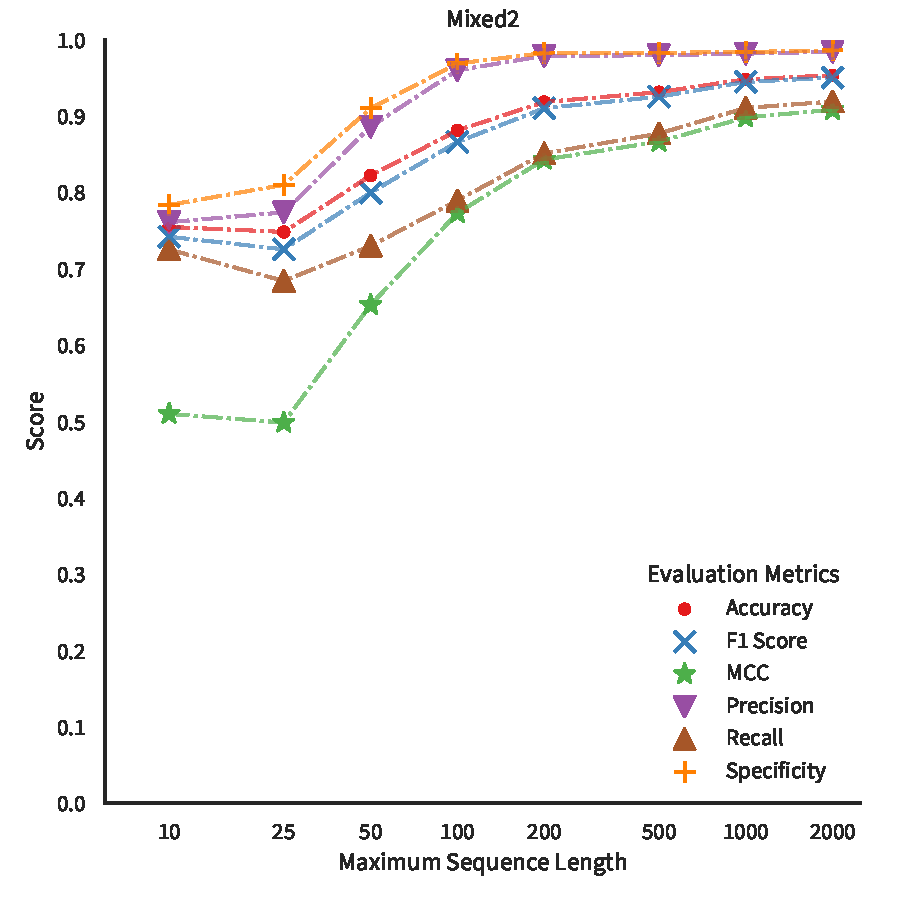
\includegraphics[width=5.5cm]{figures/dna-len-2.pdf} }}
    \caption{Results with different values for maximum sequence length $L$.}
    \label{fig:eval_seq_len}
\end{figure}

% Table for DNA permutation.
\begin{table}
\scriptsize
\caption{\label{tab:eval_permutation} Evaluation results for the string compression technique after applying random permutations to the DNA sequences in the test set.}
\begin{tabularx}{\textwidth}{{X}*{7}{c}}
\hline
\multicolumn{1}{c}{Technique} &
\multicolumn{6}{c}{Metrics} \\
\hline
 & \tiny{Accuracy} & \tiny{Precision} & \tiny{Recall} & \tiny{F-Measure} & \tiny{MCC} & \tiny{Specificity} \\
 \hline
\textbf{\texttt{Mixed1}} & & & & & & \\
String Compression - Compressed DNA Size & 0.977 & 0.986 & 0.967 & 0.976 & 0.954 & 0.987 \\
String Compression - Compression Ratio & 0.976 & 0.994 & 0.957 & 0.975 & 0.952 & 0.994 \\
\hline
\textbf{\texttt{Mixed2}} & & & & & & \\
String Compression - Compressed DNA Size & 0.968 & 0.989 & 0.944 & 0.966 & 0.936 & 0.990 \\
String Compression - Compression Ratio & 0.975 & 0.995 & 0.953 & 0.974 & 0.951 & 0.996 \\
\hline
\end{tabularx}
\end{table}

% Experiment with sequence lengths
We perform additional experiments to study the effect of the length of the DNA sequence on the final result. For the accounts in the dataset under study, the average length of the DNA sequence is $1050.29$ with the longest sequence of length $3250$. These numbers might not be representative of the real world situation. On the one hand, newer accounts may only have a few dozen posts, on the other hand, accounts that have been operational for many years may have thousands of posts. We set different limits $L = \{10, 25, 50, 100, 200, 500, 1000, 2000\} $ for the maximum length of the DNA sequence and for each account in the dataset, we pick a sub-sequence of random length between $1$ and $L$. Figure \ref{fig:eval_seq_len} shows the value for all evaluation metrics, averaged over 100 executions, with different values of $L$ when using the original DNA size and the compression ratio as the two features for training the logistic regression classifier. For short DNA sequences, say $L \le 25$, the model performs poorly in classifying the Twitter accounts and we see low scores for all evaluation metrics with MCC score as low as 0.5. However, there are great improvements in the performance as the DNA sequence length increases. We believe this is due to the fact that a longer DNA sequence potentially allows the compression algorithm to look for longer repeating patterns that can be utilised for efficient compression, hence leading to higher compression ratio for the DNA sequences of bot accounts, compared to the compression ratio for the DNA sequences of the genuine user accounts.

% Experiment with permutation of DNA sequences.
We also analyze the effectiveness of our approach against evading techniques by performing an experiment where we apply random permutations to the digital DNA sequences. We again pick $50\%$ of the accounts in the dataset for training and the keep the remaining $50\%$ for evaluation. However, before evaluating the classifier, we apply random permutations to the DNA sequences in the test set. We repeat this experiment 100 times and present the average value for the evaluation metrics in Table \ref{tab:eval_permutation}. We notice that the string compression technique still performs well and there is only a slight decrease in the performance with respect to the evaluation metrics.

% Plot for proportion of bots.
\begin{figure}
    \centering
    \subfloat[\texttt{Mixed1}]{{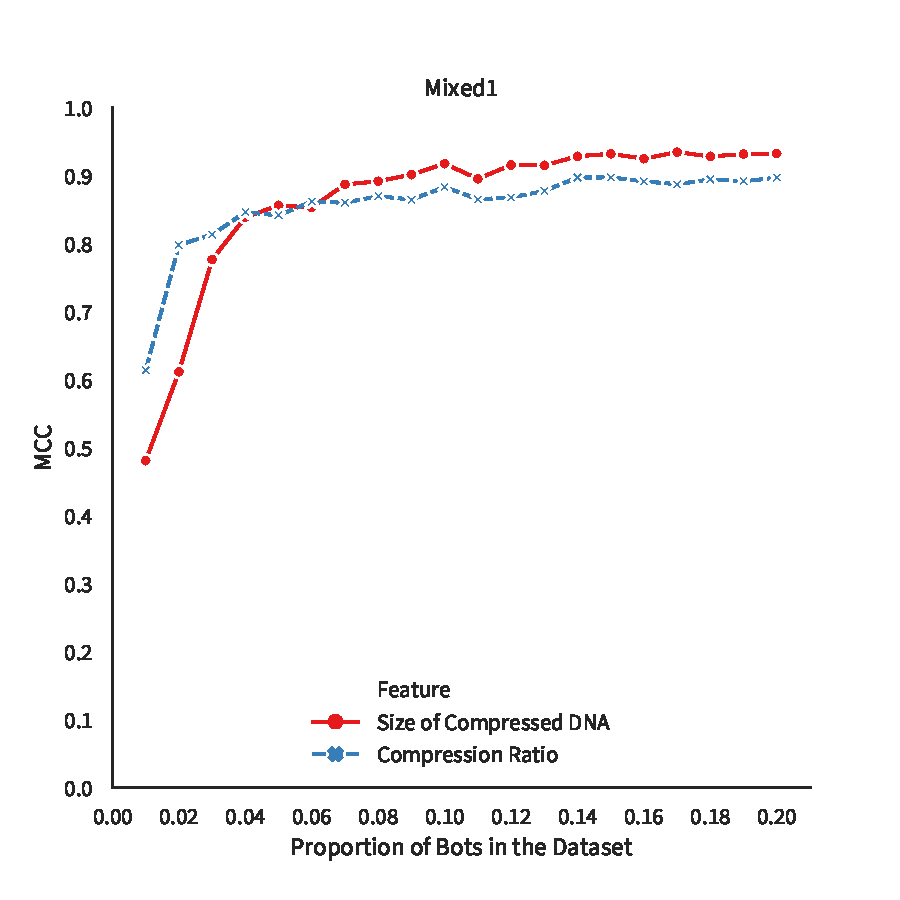
\includegraphics[width=0.47\textwidth]{figures/dna-bot-proportion-mcc-1.pdf}}}
    \qquad
    \subfloat[\texttt{Mixed2}]{{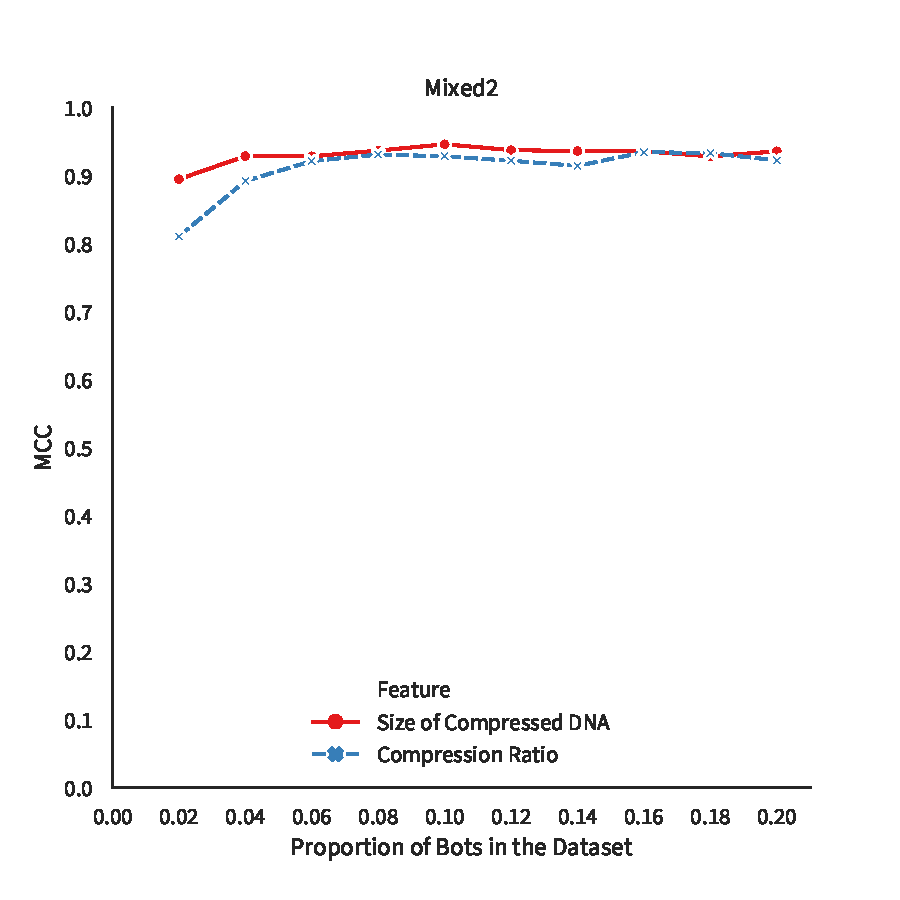
\includegraphics[width=0.47\textwidth]{figures/dna-bot-proportion-mcc-2.pdf}}}
    \caption{\label{fig:eval_proportion} Results with different proportions of bot accounts in the dataset.}
\end{figure}

% Experiment with proportion of bots in the test set.
In both \texttt{Mixed1} and \texttt{Mixed2}, about 40-50\% accounts are labelled as bots. However, the actual proportion of bots on Twitter is expected to be much smaller than this. According to a report submitted by Twitter to the United States Securities and Exchange Commission \cite{twitter_sec_2014}, less than 5\% of monthly active users (MAU) are bots. It has been estimated in \cite{varol2017online} that bots make up about 9-15\% of accounts on Twitter. We address this issue by keeping a fixed number of genuine user accounts in the test set and vary the proportion of bot accounts from 1\% to 20\%. Figure \ref{fig:eval_proportion} shows the MCC score evaluated over the different proportions of bot accounts in both \texttt{Mixed1} and \texttt{Mixed2} datasets averaged over 100 different executions. Our approach appears to be reliable even with unbalanced test sets and performs slightly worse only when the test set is extremely unbalanced with bot accounts making up only 1-2\% of the accounts.

\section{Conclusion and Future Work}
In this paper we presented an approach to detect bot accounts on the popular online social network Twitter by building on top of the already existing technique of Digital DNA. We extended the idea of using a digital DNA sequence to model the past activity of Twitter account by employing the technique of string compression on such a sequence. By leveraging the compression statistics, we were able to accurately model and visually represent the behaviour of Twitter accounts. This approach of modelling account behaviour with digital DNA is fast and can be scaled to handle large number of accounts with the advantage of being language and content independent. Our experiments suggest that this technique is also robust to potential bot evading techniques and can work with unbalanced datasets too. A future path of work can look at incorporating other user-profile and content-based features into the digital DNA sequence and apply this technique to identify automated accounts on other social media platforms such as Facebook and Reddit.

% --- ACKNOWLEDGE FUNDING SOURCES
\vspace{3mm}
\noindent\textbf{Acknowledgement.} This publication has emanated from research supported in part by a research grant from Science Foundation Ireland (SFI) under Grant Number SFI/12/RC/2289P2.

% --- BIBLIOGRAPHY
\bibliographystyle{splncs03}
\bibliography{biblio} 

\end{document}
